
\documentclass[aspectratio=169]{beamer}
\usetheme{metropolis}           % Use metropolis theme
\usepackage[utf8]{inputenc}
\usepackage{graphicx}
\usepackage{eso-pic}
\usepackage{graphics}
\usepackage{tikz}
\usepackage[export]{adjustbox}
\usepackage{multicol}
\usepackage{listings}
\usepackage{helvet}
\usepackage{booktabs}
\usepackage{threeparttable}
\usepackage{fontspec}
\usepackage{hyperref}
\hypersetup{urlcolor=DarkBlue}

\title{Topic 5 - Track 1 \newline Randomisation}
\date{\today}
\author{Author of Session here!} % Name of author(s) of session here
\institute{Development Impact Evaluation (DIME) \newline The World Bank }
\setbeamercolor{background canvas}{bg=white}	% Sets background color

% The below command places the World Bank logo and DIME logo to the right corner
\titlegraphic{%
	\begin{picture}(0,0)
	\put(330,-180){\makebox(0,0)[rt]{
\includegraphics[width=3cm]{../../img/WB_logo}}}
	\end{picture}%
	\begin{picture}(0,0)
	\put(390,-180){\makebox(0,0)[rt]{
\includegraphics[width=1.5cm]{../../img/i2i}}}
	\end{picture}%
}

%%% Section page with picture of Light bulb
\makeatletter
\defbeamertemplate*{section page}{mytheme}[1][]{
	\centering
	\begin{minipage}{22em}
		\raggedright
		\usebeamercolor[fg]{section title}
		\usebeamerfont{section title}
		\par
		\ifx\insertsubsectionhead\@empty\else%
		\usebeamercolor[fg]{subsection title}%
		\usebeamerfont{subsection title}%
		\fi
		\ifstrempty{#1}{}{%
			\includegraphics[width=100mm, height=60mm]{#1}%
		}
		\insertsectionhead\\[-1ex]
		\insertsubsectionhead
		\usebeamertemplate*{progress bar in section page}

	\end{minipage}
	\par
	\vspace{\baselineskip}
}
\makeatother

%%% Define a command to include picture in section,
%%% make section, and revert to old template
\newcommand{\sectionpic}[2]{
	\setbeamertemplate{section page}[mytheme][#2]
	\section{#1}
	\setbeamertemplate{section page}[mytheme]
}

\usepackage{fancyvrb} % Allows customization of verbatim environments
%Fancyvrb docs: http://mirrors.ibiblio.org/CTAN/macros/latex/contrib/fancyvrb/doc/fancyvrb-doc.pdf
\fvset{fontsize=\scriptsize} % The font size of all verbatim text can be changed here

%So we can use option FloatBarrier, which is similar to [H] but is an
%alternative solition when the algorithm can't solce [H] as too many
%settings are going on. [H] seems to get stuck in infinite loop
%https://tex.stackexchange.com/questions/2275/keeping-tables-figures-close-to-where-they-are-mentioned
\usepackage{placeins}
\newcommand{\codeexample}[2]{
	\begin{figure}
		\VerbatimInput[
		framesep=3mm,
		frame=lines, % line above and below code section
		numbers=left, %Line number
		label= #1, %name of code section
		baselinestretch=0.90, %Use line space more similat to line space in code editors
		]{#2} %Write the relative file path and the name of the file to be included
	\end{figure}
	\FloatBarrier
}
%% The below command creates the ligh bulb logos in the top right corner of the
\begin{document}

	{
		\usebackgroundtemplate{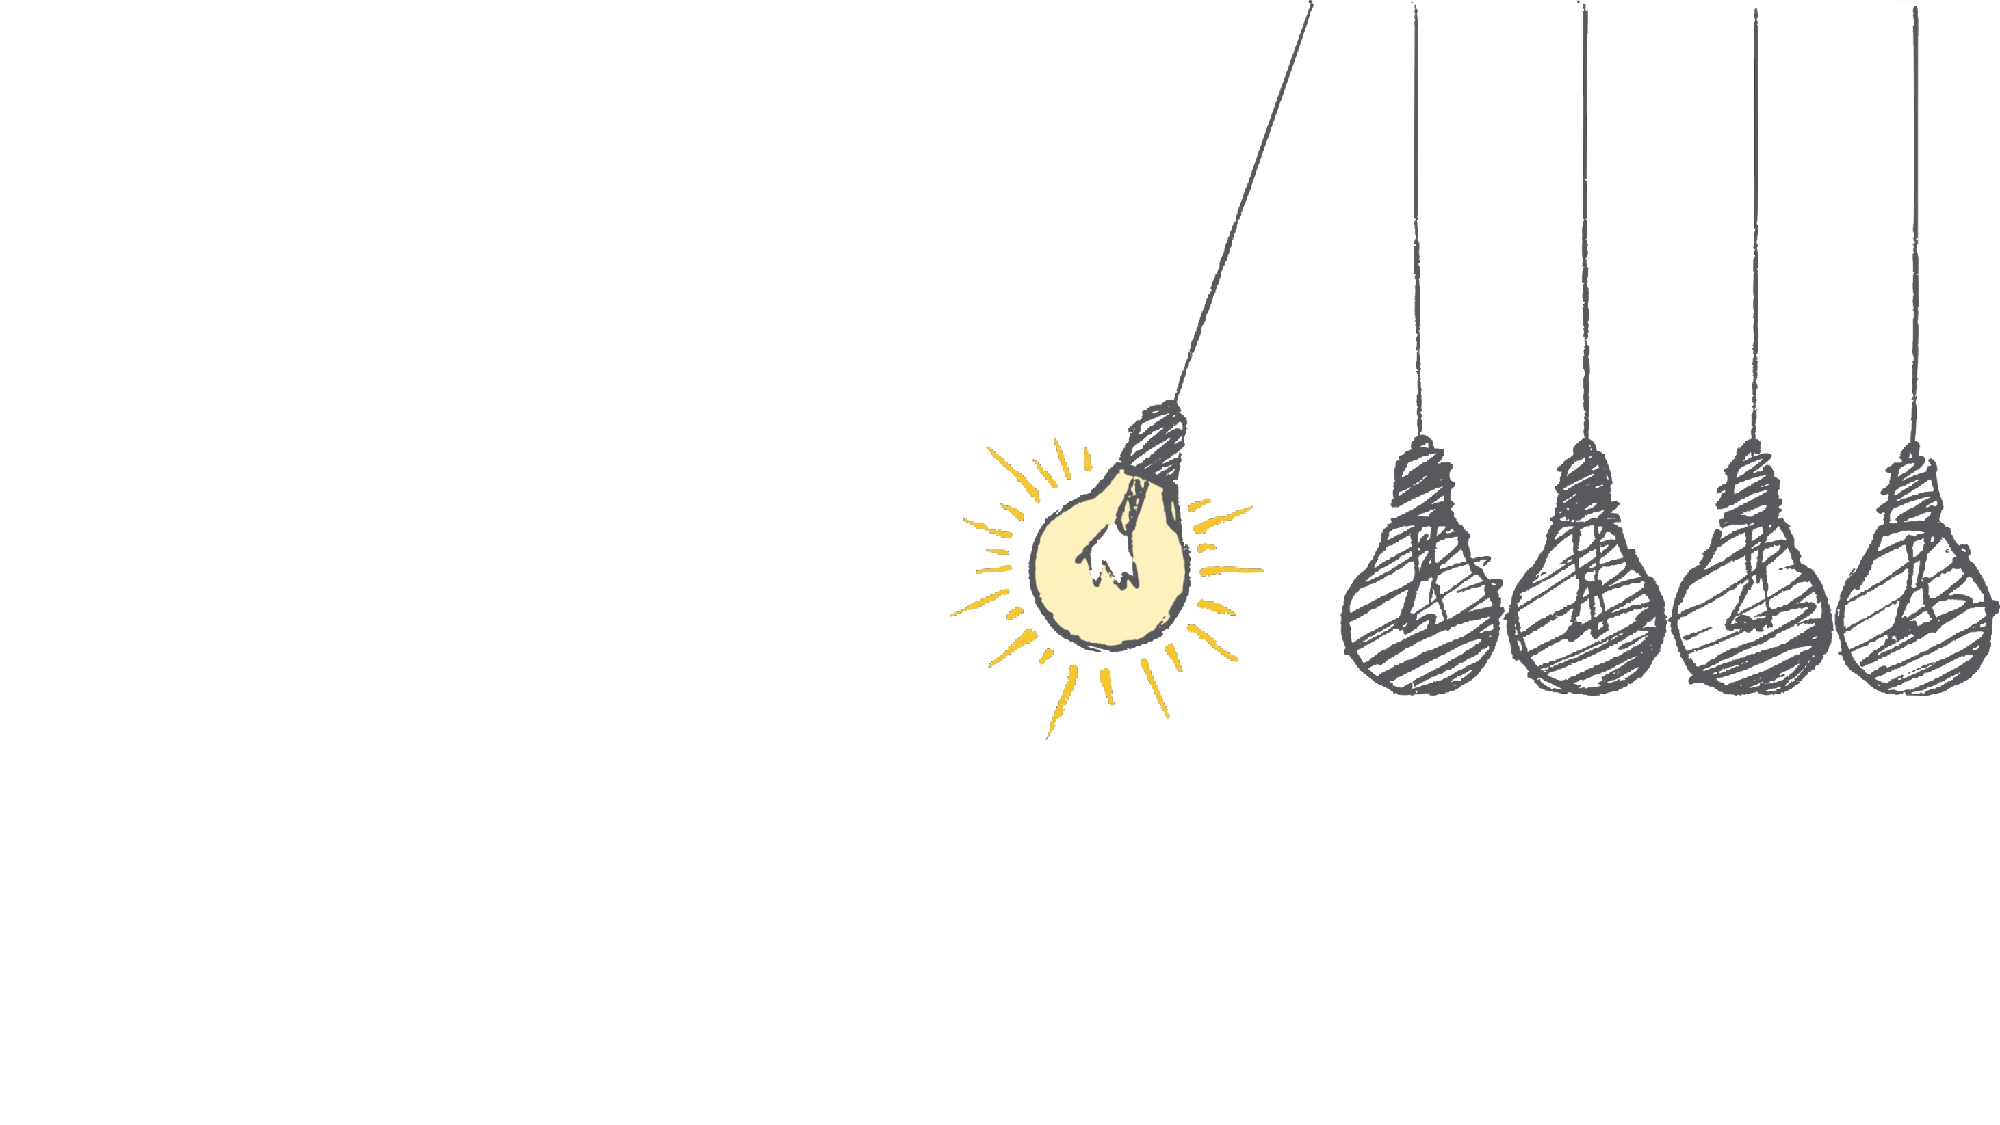
\includegraphics[height=55mm, right]{../../img/top_right_corner.pdf}}
		\maketitle
	}

%%%%%%%%%%%%%%%%%%%%%%%%%%%%%%%%%%%%%%%%%%% heading of section 1
\begin{frame}{Key Terms}
	\begin{itemize}
		\item Treatment and Control
		\begin{itemize}
			\item Treatment means receiving the project
			\item control means not receiving the project
		\end{itemize}
		\item Treatment Arms
		\begin{itemize}
			\item If there are multiple versions of the intervention, each group receiving a different version of the project is called a treatment arm.
		\end{itemize}
	\end{itemize}
\end{frame}



\begin{frame}{Types of Randomization}
	\begin{itemize}
		\item Simple
		\begin{itemize}
			\item Each individual person is assigned either T or C
		\end{itemize}
		\item Cluster
		\begin{itemize}
			\item Randomization happens on group level (village, school etc. ) and all individuals in a group are assigned the same treatment
		\end{itemize}
		\item Stratified
		\begin{itemize}
			\item Sub-sets of similar observations (rich/poor, male/female etc.) are determined in advance, and randomization is done separately within each sub-set
			\item Guarantees that equal number of similar observations (rich/poor, male/female etc.) are assigned to be each treatment and control
		\end{itemize}
		\item Pairwise
		\begin{itemize}
			\item Extreme form of stratification
			\item All units are matched to make pairs that are as similar as possible and one unit from each pair is assigned to be T or C
		\end{itemize}
	\end{itemize}
\end{frame}


\begin{frame}{Why do we randomize?}
	\begin{itemize}
		\item “Random” does not imply “completely random”, we want a controlled and replicable randomization
		\item We want to assign the intervention of our projects so that the control group is as similar as possible to the treatment group as possible
		\begin{itemize}
			\item This is called a balance treatment assignment
			\item Randomization is the most common tool to achieve that
		\end{itemize}
		\item Each observation needs to have the same probability to end up in the each treatment arm, and all members in a strata need to be statistically similar
	\end{itemize}
\end{frame}


\begin{frame}{Methods of randomization}
	\begin{itemize}
		\item Good:
		\begin{itemize}
			\item Field Based
			\item Stata, R, Python – and other replicable software
		\end{itemize}
		\item Bad:
		\begin{itemize}
			\item Excel – and other non-replicable software
			\item Excel and many other software has random generators, but they do not allow a controlled randomization
		\end{itemize}
	\end{itemize}
\end{frame}

\begin{frame}{Method: Field Based}
	\begin{itemize}
		\item Examples
		\begin{itemize}
			\item Drawing numbers from a hat, flipping a coin etc.
		\end{itemize}
		\item Advantage
		\begin{itemize}
			\item Transparent to participants
			\item Allows randomization without exactly knowing treatment population in advance
		\end{itemize}
		\item Disadvantages
		\begin{itemize}
			\item Not transparent to anyone not present
			\item Not replicable
			\item Difficult to manage any a complex randomization with, for example, stratification
		\end{itemize}
	\end{itemize}
\end{frame}



\begin{frame}{Method: Stata}
	\begin{itemize}
		\item Advantages
		\begin{itemize}
			\item Fully replicable
			\item Relatively easy to set up complex randomizations
			\item We can run a test randomization and analyze the outcome before we draw new random numbers for the actual randomization
		\end{itemize}
		\item Disadvantages
		\begin{itemize}
			\item Can seem very mysterious to beneficiaries and project staff
		\end{itemize}
	\end{itemize}
\end{frame}



\begin{frame}{Prepare randomization in Stata}
	\begin{itemize}
		\item Obtain a list of observations to be randomized
		\item Define a randomization rule
		\begin{itemize}
			\item How many units (people) are in the population?
			\item How many treatment arms do you have?
			\item How big share of the observations should end up in each group?
			\item Are we using stratification?
			\item Which variables will we use to test balance?
		\end{itemize}
		\item Randomize and document using Stata!
	\end{itemize}
\end{frame}



\begin{frame}{Ex 1: Basic Randomization in Stata}
	\begin{itemize}
		\item We have 10 students and we want half of them to be treatment and control
		\item What is our randomization rule?
		\item How do we do this in Stata so it is random but replicable?
	\end{itemize}
\end{frame}


\begin{frame}[fragile]{Ex 1: Basic Randomization in Stata}
	\begin{columns}[c]
		\column{.60\textwidth}
		\begin{figure}
			\centering
			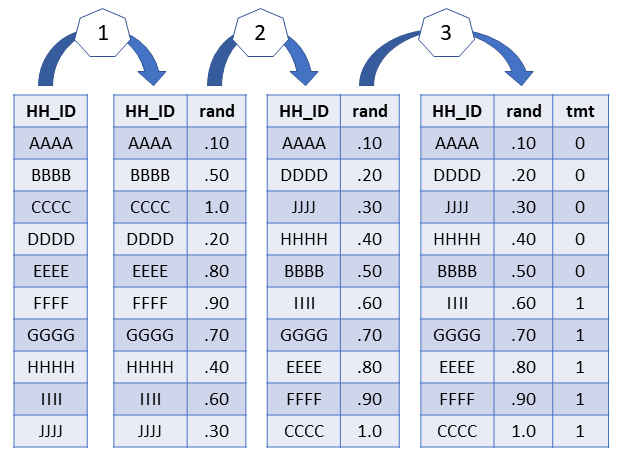
\includegraphics[width=\linewidth]{img/randomeg1}
		\end{figure}

		\column{.40\textwidth}
		\begin{enumerate}
			\item \small Start with a sorted list of observations you want to randomize. Generate a random number.
			\item \small Sort the observations after this random number. The order of the observations are now randomly sorted.
			\item \small Assign 0 (control) to the first half of the observations, and assign 1 (treatment) to the second half.
		\end{enumerate}
	\end{columns}
\end{frame}


\begin{frame}{The 3 rules of replicable randomization}
	\begin{itemize}
		\item We want to be able to replicate the randomization and get the same results each time. This is needed for research transparency
		\item To achieve that in Stata we have three rules:
		\begin{itemize}
			\item Set the version of Stata
			\item Set the seed
			\item Stable sort
		\end{itemize}
		\item The next slides explains the meaning of these rules and why it matters
	\end{itemize}
\end{frame}


\begin{frame}{Rule 1: Set the version of Stata}
	\begin{columns}[c]
		\column{.60\textwidth}
		\begin{figure}
			\centering
			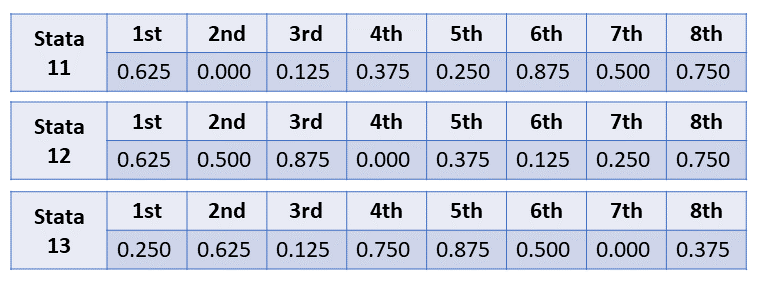
\includegraphics[width=\linewidth]{img/rand-version.png}
		\end{figure}
		\column{.40\textwidth}
		\begin{itemize}
			\item \small Stata has pre-calculated list of random numbers. However, these lists differs between versions of Stata.
			\item \small In reality these lists are billions of items long, instead of 8 as in the example above
			\item \small For our purposes, all these lists are equally good, but we need to pick one, and always use the same one. You can set Stata to use an older list but not a newer
		\end{itemize}
	\end{columns}
\end{frame}

\begin{frame}{Rule 1: Set the version of Stata}
	\begin{columns}[c]
		\column{.65\textwidth}
		\begin{figure}
			\centering
			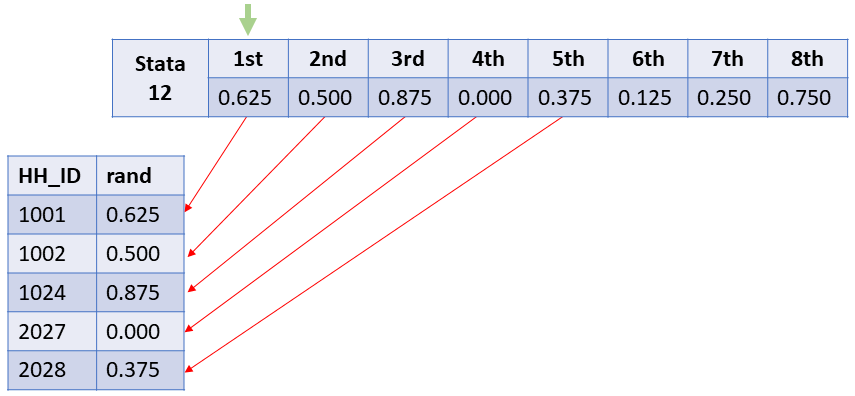
\includegraphics[width=\linewidth]{img/rule1}
		\end{figure}
		\column{.35\textwidth}
		\begin{itemize}
			\item \small Stata goes through the lists and assigns the 1st value to the first observation, 2nd to the second observation, etc.
		\end{itemize}
	\end{columns}
\end{frame}


\begin{frame}{Rule 2: Set the seed}
	\begin{columns}[c]
		\column{.65\textwidth}
		\begin{figure}
			\centering
			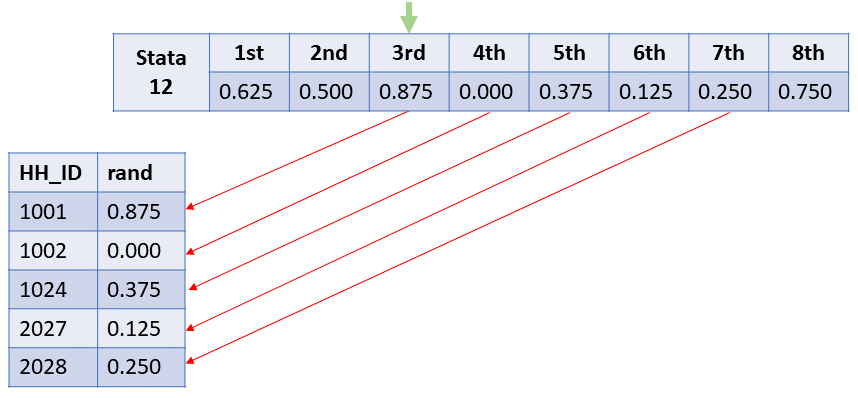
\includegraphics[width=\linewidth]{img/rule2}
		\end{figure}
		\column{.35\textwidth}
		\begin{itemize}
			\item \small Setting the seed change the starting place in the list
			\item \small Randomly selecting a seed means randomizing the starting point
			\item \small If no seed is set, a seed is randomized each time you run the code, this means random but not replicable
		\end{itemize}
	\end{columns}
\end{frame}


\begin{frame}{Rule 3: Stable sort}
	\begin{columns}[c]
		\column{.65\textwidth}
		\begin{figure}
			\centering
			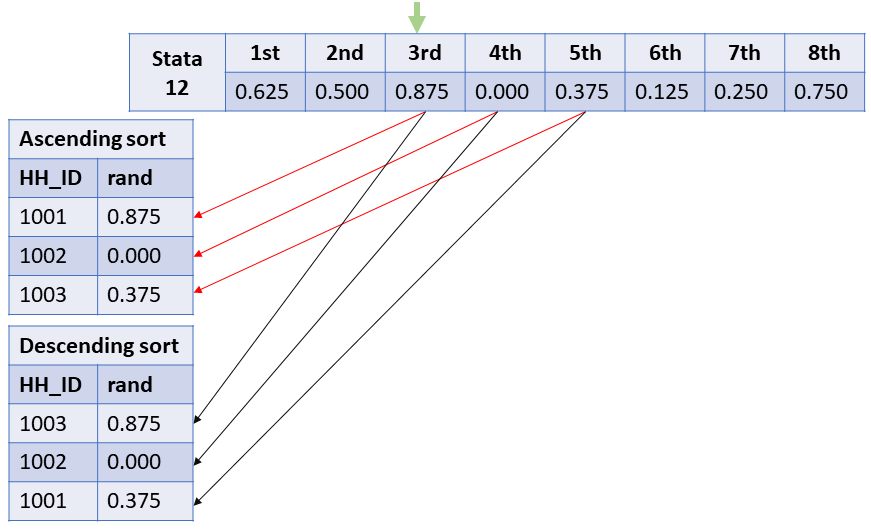
\includegraphics[width=\linewidth]{img/rule3}
		\end{figure}
		\column{.35\textwidth}
		\begin{itemize}
			\item \small The two data sets to the left are sorted differently, and while the same random numbers were picked, the result of the randomization is different.
			\item \small Adding and removing observations can change the sort order
		\end{itemize}
	\end{columns}
\end{frame}


\begin{frame}{The 3 rules of replicable randomization}
	\begin{itemize}
		\item Set the version of Stata
		\begin{itemize}
			\item Guarantees the same list of random numbers
			\item See commands ieboilstart or version in Stata
		\end{itemize}
		\item Set the seed
		\begin{itemize}
			\item 	Guarantees the same starting point in that list
			\item See command set seed. Randomize a seed at least 6 digits long (for example at \url{www.random.org})
		\end{itemize}
		\item Stable sort
		\begin{itemize}
			\item Guarantees that the same observation gets the same random number from the list
			\item Sort the data in way that will remain constant even if someone else change the sort order of the data set you are using
			\item Be aware that changing the data set, adding or removing observations, changes the sort order!
		\end{itemize}
	\end{itemize}
\end{frame}



\begin{frame}{Ex 1: Basic Randomization in Stata}
	\begin{itemize}
		\item Open \texttt{endline\_data\_raw.dta}
		\item We have 1067 households and we want half of them to be treatment and control
		\item What is our randomization rule?
		\item Let’s see an example of a replicable randomization of this
	\end{itemize}
\end{frame}


\begin{frame}{Ex 1: Basic Randomization in Stata - Step 1}
	Apply the three rules of randomization. Can you spot them?
	\codeexample{randomization-1.do}{code/randomization-1.do}
\end{frame}

\begin{frame}{Ex 1: Basic Randomization in Stata - Step 2}
	After the three rules are set, generate treatment variable
	\codeexample{randomization-2.do}{code/randomization-2.do}
\end{frame}

\begin{frame}{Ex 2: Multi-Arm Randomization in Stata}
	\begin{itemize}
		\item Multiple treatment arms
		\item We have 1067 households and we want one third of them to be control and two treatment arms with one third in each
	\end{itemize}
\end{frame}

\begin{frame}{Ex 2: Multi-Arm Randomization in Stata - Step 1}
	Start over and apply the three rules again
	\codeexample{randomization-1.do}{code/randomization-1.do}
\end{frame}

\begin{frame}{Ex 2: Multi-Arm Randomization in Stata - Step 1}
	\codeexample{randomization-multi-arm.do}{code/randomization-multi-arm.do}
\end{frame}


\begin{frame}{Real life issues}
	\begin{itemize}
		\item The example we have covered here is a school book example, but in real life, there are many common issues that makes randomization more complicated
		\item There are commands that take care of these types of issues. Among them we recommend \texttt{randtreat}. To use this in a real life example, see track 2
		\item But if you do not understand the school book example, you are likely to not know how to use \texttt{randtreat} properly
	\end{itemize}
\end{frame}


\begin{frame}{Common Issues}
	\begin{itemize}
		\item Differently sized groups. For example 40\% is control, and treatment arm 1 and 2 is 30\% each – \texttt{randtreat} solves this
		\item Stratification. Split up the observations into groups. Rich/Poor, Male/Female, regions, etc. and then do the randomization in each group – \texttt{randtreat} solves this
		\item Uneven groups (for example, divide 20 observations in 8 groups). The number of observations is not evenly divisible with the number of treatment arms. How to deal with the left overs observation? All to control? All to treatment? – \texttt{randtreat} solves this
	\end{itemize}
\end{frame}



\begin{frame}{The 3 rules still apply to randtreat}
	\begin{itemize}
		\item Even if you are using \texttt{randtreat} you need to remember to apply the three rules for the randomization to be fully replicable:
		\begin{itemize}
			\item Version
			\item Seed
			\item Sort
		\end{itemize}
	\end{itemize}
\end{frame}


\begin{frame}{Additional Resources}
	\begin{itemize}
		\item Duflo, Glennerster, and Kremer Handbook
		\begin{itemize}
			\item Useful for understanding types of randomization and reasons for randomizing
			\item \url{http://economics.mit.edu/files/806}
		\end{itemize}
	\end{itemize}
\end{frame}


%%%%%%%%%%%%%%%%%%%%%%%%%%%%%%%%%%%%%%%%%%% Final thougts section
\begin{frame}{Conclusion}


\vspace{20mm}
For more information or further questions please contact:
\newline John Doe (\url{johndoe@worldbank.org}) \newline Mary Doe (\url{marydoe@worldbank.org})

\end{frame}

%%%%%%%%%%%%%%%%%%%%%%%%%%%%%%%%%%%%%%%%%%% The End
\sectionpic{Thank You!}{../../img/section_slide}






\end{document}
